\subsection{Near field}

\begin{frame}{Near field}
    \begin{columns}
        \column{0.6\textwidth}
        Condition: \( \beta r \ll 1 \) or \( r \ll \lambda \). 
        \begin{itemize}
            \item Electromagnetic fields:
        \end{itemize}
        \begin{align*}
            \mathbf{H} &= \dfrac{ I L \exp ( -j \beta r ) }{4 \pi r^2} \sin \theta \mathbf{ \hat{\phi} }, \\
            \mathbf{E} &= - j \eta \dfrac{I L}{4 \pi \beta} \dfrac{\exp ( - j \beta r )}{r^3} \left( \sin \theta \mathbf{ \hat{\theta} } + 2 \cos \theta \mathbf{ \hat{r} } \right).
        \end{align*}
        \begin{itemize}
            \item Poynting vector:
        \end{itemize}
        \begin{equation*}
           \mathbf{S} = - \dfrac{ j \eta }{2 \beta} \left( \dfrac{I L}{4 \pi} \right)^2 \dfrac{1}{r^5} \left( \sin^2 \theta \mathbf{\hat{r}} - \sin 2 \theta \mathbf{\hat{\theta}} \right). 
        \end{equation*}
        
        \vspace{3mm}
        Power transfer by mutual induction.
        \column{0.4\textwidth}
        Near field properties:
        \begin{itemize}
            \item Electrostatic field.
            \item No Radiation Loss.
        \end{itemize}
        \begin{figure}
            \centering
            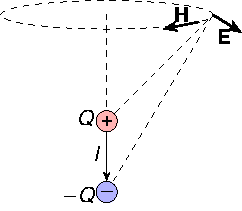
\includegraphics{Figures/Electrostatic_dipole.pdf}
            \caption{Electrostatic dipole model.}
            \label{fig:Electrostatic_diople}
        \end{figure}
    \end{columns}
\end{frame}

